\begin{columns}[T] % align columns
  \begin{column}{.45\textwidth}   
    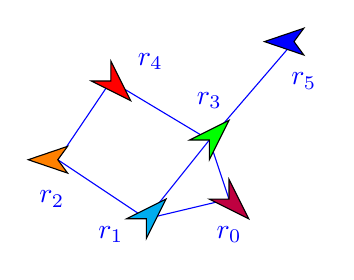
\begin{tikzpicture}
      \draw [color=blue] (4,4) -- (3.2,3); % r1--r3
      \draw [color=blue] (4,4) -- (5.075,5.25); %r3--r5
      \draw [color=blue] (4,4) -- (2.75,4.75); % r3--r4
      \draw [color=blue] (4,4) -- (4.25, 3.25); %r3--r0
      \draw [color=blue] (2.75,4.75) -- (2.075,3.75); % r4--r2
      \draw [color=blue] (3.2,3) -- (2.075,3.75); % r1--r2
      \draw [color=blue] (3.2,3) -- (4.25,3.25); %r1--r0
      \draw[fill=red] (3,4.5) -- (2.75,5) -- (2.75,4.75) -- (2.5,4.75)   -- cycle;
      \node[color=blue] at (3.25, 5) {$r_4$};
      \draw[fill=blue] (5.2,5.42) -- (4.7,5.25) -- (5.2,5.08) -- (5.075,5.25)  -- cycle;
      \node[color=blue] at (5.2,4.75) {$r_5$};
      \draw[fill=green] (4,4) -- (3.75,4) -- (4.25,4.25) -- (4,3.75) -- cycle;
      \node[color=blue] at (4, 4.5) {$r_3$};
      \draw[fill=orange] (2.2,3.92) -- (1.7,3.75) -- (2.2,3.58) -- (2.075,3.75)  -- cycle;
      \node[color=blue] at (2, 3.25) {$r_2$};
      \draw[fill=cyan] (3.2,3) -- (2.95,3) -- (3.45,3.25) -- (3.2,2.75)  -- cycle;
      \node[color=blue] at (2.75, 2.8) {$r_1$};
      \draw[fill=purple] (4.5,3) -- (4.25,3.5) -- (4.25,3.25) -- (4,3.25)   -- cycle;
      \node[color=blue] at (4.25, 2.8) {$r_0$};    
    \end{tikzpicture}
  \end{column}%
  \begin{column}{.45\textwidth}
    \begin{tikzpicture}
      \tikzstyle{every state}=[fill=purple!50, draw=none]
      \node[state, scale=0.7] (A) at (2,3) {\large{$r_5$}};
      \node[state, scale=0.7] (B) at (2,2) {\large{$r_3$}};
      \node[state, scale=0.7] (C) at (2,1) {\large{$r_1$}};
      \node[state, scale=0.7] (D) at (1,1) {\large{$r_0$}};
      \node[state, scale=0.7, fill=orange!50] (E) at (3,1) {\large{$r_4$}};
      \node[state, scale=0.6, fill=orange!50] (F) at (4,0.5) {\large{$r_2$}};
      \draw[arc] (A) to[out=-90, in=90] (B);
      \draw[arc] (B) to[out=-90, in=90] (C);
      \draw[arc] (B) to[out=-135, in=45] (D);
      \draw[arc] (B) to[out=-45, in=135] (E);
      \draw[arc] (E) to[out=-25, in=150] (F);
    \end{tikzpicture}

  \end{column}%
\end{columns}


%\caption{[left] Communication graph of six robots. [right] Assume
%% $r_5$ has the highest stable ID and a vacancy. A spanning tree
%% corresponding to the left communication graph is built, in which the
%% root is $r_5$. Let $r_4$ be the relocate robot, it then is the root
%% of the moving subtree, in which $r_2$ is its descendant.}
